\noindent

\includegraphics[height=1.25cm]{images/pictograms/benchmark}

\includegraphics[height=1.25cm]{images/pictograms/under_construction}

\includegraphics[height=1.25cm]{images/pictograms/FDM}

\includegraphics[height=1.25cm]{images/pictograms/paraview}
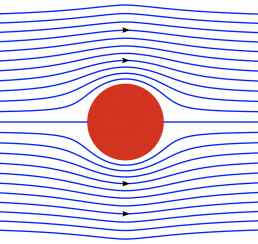
\includegraphics[height=1.25cm]{images/pictograms/streamfunction}


%%%%%%%%%%%%%%%%%%%%%%%%%%%%%%%%%%%%%%%%%%%%%%%%%%%%%%%%%%%%%%%%%%%%%%%%%%%%%%%%%%%%%%%%%%%%%%%%%%%

\begin{flushright} {\tiny {\color{gray} python\_codes/fieldstone\_153/text.tex}} \end{flushright}

%\lstinputlisting[language=bash,basicstyle=\small]{python_codes/template_keywords.key}

\par\noindent\rule{\textwidth}{0.4pt}

\begin{center}
\inpython
{\small Code: \url{https://github.com/cedrict/fieldstone/tree/master/python_codes/fieldstone_153}}
\end{center}

\par\noindent\rule{\textwidth}{0.4pt}

%{\sl This stone was developed in collaboration with Donald Duck}. \index{contributors}{D. Duck}
%\par\noindent\rule{\textwidth}{0.4pt}

%{\bf \color{teal} Purpose}: implement and document bla bla 

%\par\noindent\rule{\textwidth}{0.4pt}

%%%%%%%%%%%%%%%%%%%%%%%%%%%%%%%%%%%%%%%%%%%%%%%%%%%%%%%%%%%%%%%%%%%%%%%%%%%%%%%%%%%%%%%%%%%%%%%%%%%

The theory and derivations of the vorticity-stream function approach is 
presented in detail in Chapter~\ref{MMM-chapt:streamfunction}.

We start from the Poisson equation for the vorticity $\omega$
\begin{equation}
\vec\nabla^2 \omega = -\frac{1}{\eta_0} \left( -\frac{\partial (\rho g_x)}{\partial y}
+\frac{\partial (\rho g_y)}{\partial x} \right)
\end{equation}
In what follows we assume that the domain is a Cartesian box aligned 
with the $x,y$ axis. The gravity is constant and vertical so that $g_x=0$ and
then 
\begin{equation}
\vec\nabla^2 \omega 
= -\frac{g_y}{\eta_0} 
\frac{\partial \rho}{\partial x} 
\end{equation}

As shown in Section~\ref{MMM-ss:fdm_diff2D}, the Laplacian of $\omega$
can be discretised with a second order central difference stencil:
\[
\vec\nabla^2 \omega |_{i,j} 
= \frac{\omega_{i+1,j} -2\omega_{i,j} + 2\omega_{i-1,j}}{h_x^2}
+ \frac{\omega_{i,j+1} -2\omega_{i,j} + 2\omega_{i,j-1}}{h_y^2}
+{\cal O}(h_x^2,h_y^2)
\]
while the density gradient is approximated by a second order
central difference:
\[
\frac{\partial \rho}{\partial x}|_{i,j} 
= \frac{\rho_{i+1,j}-\rho_{i-1,j}}{2 h_x} + {\cal O}(h_x^2)
\]
In the end, 
\[
\frac{\omega_{i+1,j} -2\omega_{i,j} + 2\omega_{i-1,j}}{h_x^2}
+ \frac{\omega_{i,j+1} -2\omega_{i,j} + 2\omega_{i,j-1}}{h_y^2}
= -\frac{g_y}{\eta_0} 
\frac{\rho_{i+1,j}-\rho_{i-1,j}}{2 h_x} 
\]
We then define the global indices
\begin{eqnarray}
k  &=& j \cdot nnx + i \nn\\
k_E &=& j \cdot nnx + i+1 \nn\\
k_W &=& j \cdot nnx + i-1 \nn\\
k_N &=& (j+1) \cdot nnx + i \nn\\
k_S &=& (j-1) \cdot nnx + i \nn
\end{eqnarray}
so that 
\[
\frac{\omega_{k_E} -2\omega_{k} + 2\omega_{k_W}}{h_x^2}
+ 
\frac{\omega_{k_N} -2\omega_{k} + 2\omega_{k_S}}{h_y^2}
= -\frac{g_y}{\eta_0} 
\frac{\rho_{k_E}-\rho_{k_W}}{2 h_x} 
\]
or, 
\[
\frac{\omega_{k_E}}{h_x^2}+
\frac{\omega_{k_W}}{h_x^2}+
\frac{\omega_{k_N}}{h_y^2}+
\frac{\omega_{k_S}}{h_y^2}-
\left(\frac{2}{h_x^2} + \frac{2}{h_y^2} \right) \omega_k
= -\frac{g_y}{\eta_0} 
\frac{\rho_{k_E}-\rho_{k_W}}{2 h_x} 
\]
This stencil is used for all interior nodes. All nodes on the boundaries 
have $\omega=0$.

Having obtained $\omega$ we can solve for $\Psi$ by solving
$\vec\nabla^2 \Psi = -\omega$.
Finally we can recover the velocity field with $u=\partial_y \Psi$ and $v=-\partial_x \Psi$.
Once again using a second order centered approach for the internal nodes:
\[
u_{i,j} = \frac{\Psi_{i,j+i}-\Psi_{i,j-i}}{2 h_y}
\]
\[
v_{i,j} = - \frac{\Psi_{i+1,j}-\Psi_{i-1,j}}{2 h_x}
\]
For the nodes on the boundary we see that these formulations are not suited:
indeed, for example, if $j=0$ (bottom boundary), then $u$ is not zero (free slip b.c.)
and should be computed, but in the equation above we find the term $\Psi_{i,j-1}$ 
which is undefined. In the end, 
for each node on the boundary we use a first order stencil that uses only 
internal nodes.

%%%%%%%%%%%%%%%%%%%%%%%%
\section*{Experiment 1}

The domain is a square of size 600~\si{\km}.  
It contains two fluids, the `mantle'  and the `slab'. 
The mantle has a density of 3200~\si{\kg\per\cubic\meter} 
and fills the domain except for a circle (the slab) of radius 100~\si{\km} 
centered at $x=L_x/2$ and $y=\frac23 L_y$  of density 
3300~\si{\kg\per\cubic\meter}. $g_0=10~\si{\meter\per\square\second}$ 
and $\eta_0=10^{21}~\si{\pascal\second}$.

\begin{center}
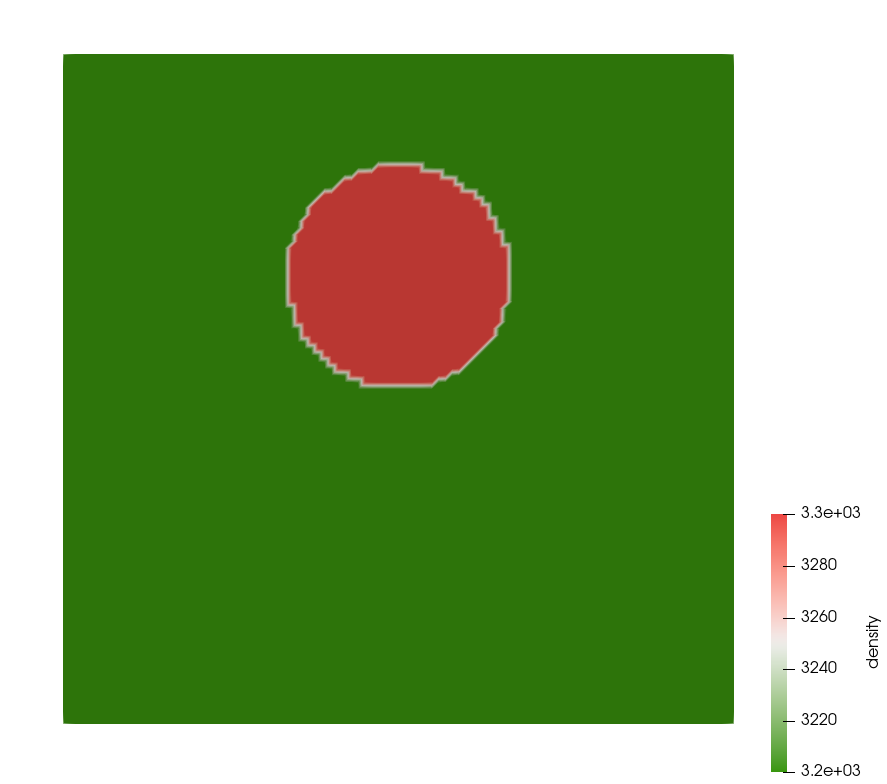
\includegraphics[width=8cm]{python_codes/fieldstone_153/results/exp1/rho}
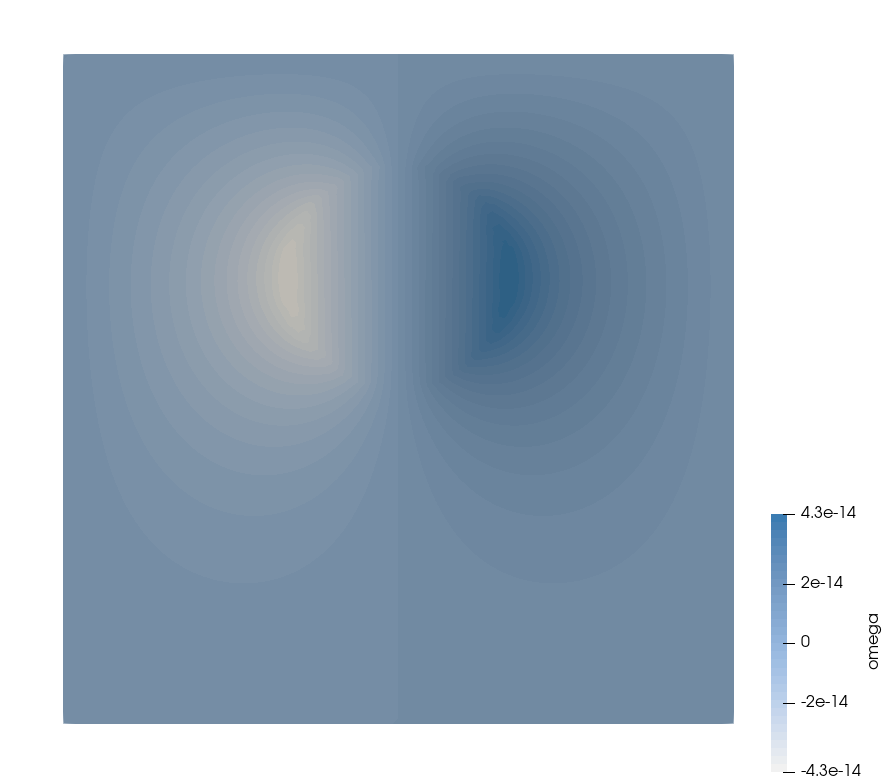
\includegraphics[width=8cm]{python_codes/fieldstone_153/results/exp1/omega}\\
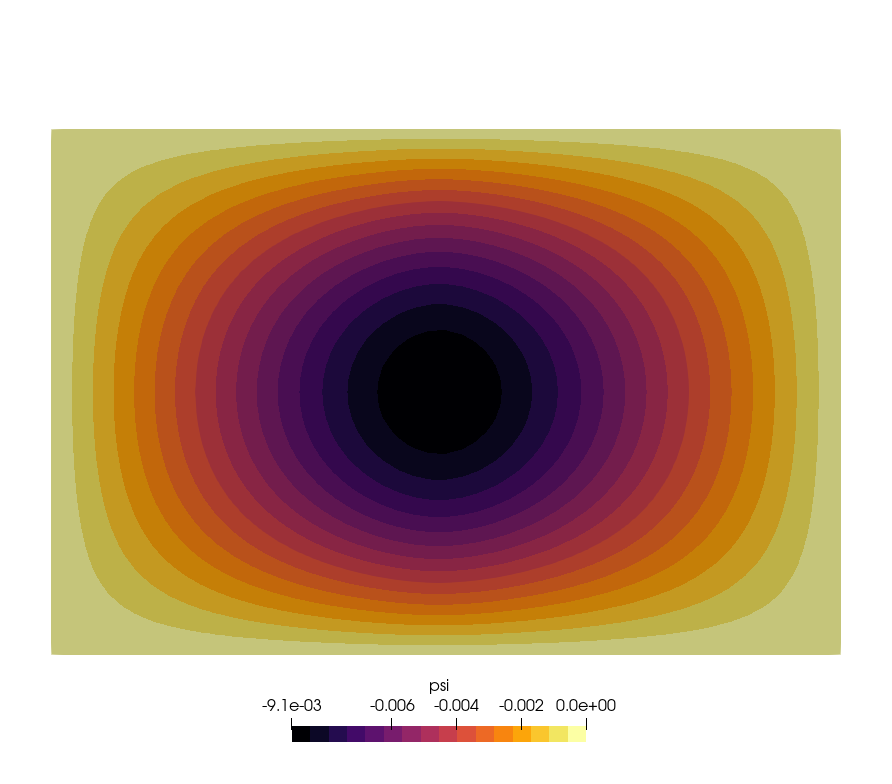
\includegraphics[width=8cm]{python_codes/fieldstone_153/results/exp1/psi}
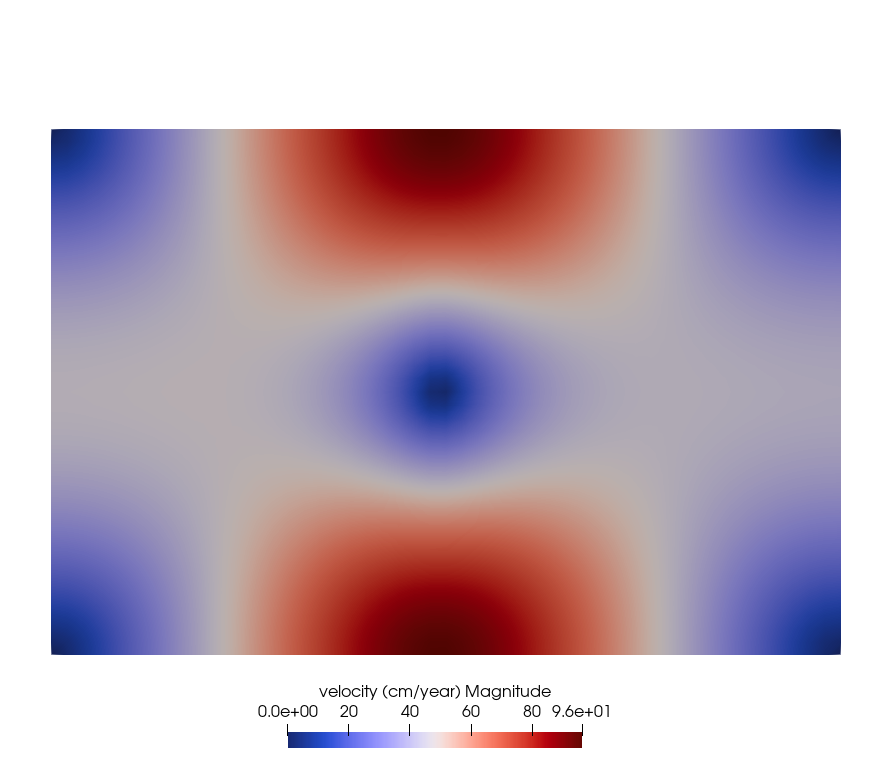
\includegraphics[width=8cm]{python_codes/fieldstone_153/results/exp1/vel}\\
{\captionfont Obtained on 101x101 mesh.} 
\end{center}



%%%%%%%%%%%%%%%%%%%%%%%%
\section*{Experiment 2}

This is inspired by Exercise 5.2 of \textcite{gery19book} which reads as 
follows:

Solve the momentum and continuity equations with finite differences using the stream
function-vorticity formulation 
on a regular grid of $51\times 41$ points. 
%({\color{teal} minus sign issue?!}):
%\[
%\Delta \omega = \frac{1}{\eta} (\partial_x \rho g_y- \partial_y \rho g_x)
%\qquad
%\omega = \Delta \Psi
%\]

Program a numerical model for buoyancy-driven flow in a vertical 
gravity field ($g_x=0$, $g_y=10~\si{\meter\per\square\second}$) 
for a density structure with two vertical layers 
(3200~\si{\kg\per\cubic\meter} and 3300~\si{\kg\per\cubic\meter} 
for the left and right layers, respectively). The model size is 
$1000~\si{\km} \times 1500~\si{\km}$.
Use a constant viscosity $\eta = 10^{21}~\si{\pascal\second}$ 
for the entire model.

\begin{center}
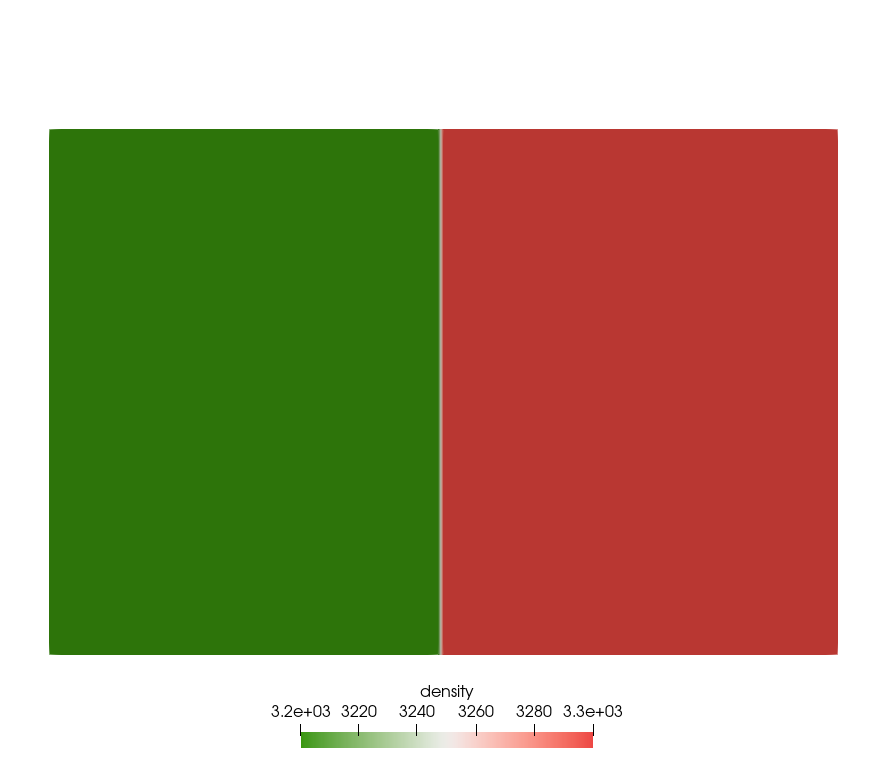
\includegraphics[width=7cm]{python_codes/fieldstone_153/results/exp2/rho}
\end{center}

Compose a matrix of coefficients $\K$ and a right hand side vector $\vec{b}$ 
and obtain the solution vector $\vec{X}$ 
for the two Poisson equations (first for $\omega$, then for $\Psi$). 

%A finite difference representation of the Poisson equations
%in 2D can be formulated as follows:
%\[
%\frac{\omega_{i,j-1}-2\omega_{i,j}+\omega_{i,j+1}}{h_x^2}
%+
%\frac{\omega_{i-1,j}-2\omega_{i,j}+\omega_{i+i,j}}{h_y^2}
%= \frac{g_y}{\eta} \frac{\rho_{i,j+1}-\rho_{i,j-1}}{2 h_x}
%\]
%\[
%\frac{\Psi_{i,j-1}-2\Psi_{i,j}+\Psi_{i,j+1}}{h_x^2}
%+
%\frac{\Psi_{i-1,j}-2\Psi_{i,j}+\Psi_{i+i,j}}{h_y^2}
%= \omega_{i,j}
%\]
%or,
%\[
%\frac{\omega_{i,j-1}}{h_x^2} 
%+\frac{\omega_{i,j+1}}{h_x^2}
%+\frac{\omega_{i-1,j}}{h_y^2}
%+\frac{\omega_{i+i,j}}{h_y^2}
%-\left(\frac{2}{h_x^2} + \frac{2}{h_y^2} \right)\omega_{i,j}
%=
%= \frac{g_y}{\eta} \frac{\rho_{i,j+1}-\rho_{i,j-1}}{2 h_x}
%\]

Use $\omega = 0$ and $\Psi = 0$ as boundary conditions for all 
external nodes of the grid.
Note that velocity components should only be computed for the internal 
nodes of the grid (i.e. for 49$\times$39 points).

%After obtaining the solution for the stream function, convert it into 
%the velocity field using finite differences 
%\[
%u_{i,j}=\frac{\Psi_{i+1,j}-\Psi_{i-1,j}}{2 h_y} 
%\qquad
%v_{i,j}=-\frac{\Psi_{i,j+1}-\Psi_{i,j-1}}{2 h_x} 
%\]

The MATLAB code of the book is reproduced hereafter: 
\begin{lstlisting}
xsize=1000000; % Horizontal
ysize=1500000; % Vertical
xnum=41; % Horizontal
ynum=31; % Vertical
xstp=xsize/(xnum-1); % Horizontal
ystp=ysize/(ynum-1); % Vertical
eta=1e+21;
gy=10; % m/s^2

% Making vectors for nodal points positions
x=0:xstp:xsize; % Horizontal
y=0:ystp:ysize; % Vertical

% Creating array for density structure (two vertical layers)
rho=zeros(ynum,xnum);
for i=1:1:ynum
  for j=1:1:xnum
    % Horizontal position of the nodal point
    if(x(j)<xsize/2)
        rho(i,j)=3200;  % left layer
    else
        rho(i,j)=3300;  % right layer
    end
  end
end

% Matrix of coefficients initialization
L=sparse(xnum*ynum,xnum*ynum);
R=zeros(xnum*ynum,1);

% Solving Poisson equation for worticity
% d2OMEGA/dx2+d2OMEGA/dy2=gy*dRHO/dx
% Composing matrix of coefficients L()
% and vector (column) of right parts R()
% Boundary conditions: OMEGA=0
% Process all Grid points
for i=1:1:ynum
  for j=1:1:xnum
    % Global index for current node
    k=(j-1)*ynum+i;
    %Boundary nodes OMEGA=0
    if(i==1 || i==ynum || j==1 || j==xnum)
        L(k,k)=1;
        R(k,1)=0;
    %Internal nodes
    else
        %Left part: d2OMEGA/dx2+d2OMEGA/dy2
        L(k,k-ynum)=1/xstp^2;
        L(k,k-1)=1/ystp^2;
        L(k,k)=-2/xstp^2-2/ystp^2;
        L(k,k+1)=1/ystp^2;
        L(k,k+ynum)=1/xstp^2;
        % Right part: gy*dRHO/dx
        R(k,1)=gy/eta*(rho(i,j+1)-rho(i,j-1))/2/xstp;
    end
  end
end
   
%Obtaining vector of solutions S()
S=L\R;

% Reload solutions S() to 2D vorticity array OMEGA()
OMEGA=zeros(ynum,xnum);
% Process all Grid points
for i=1:1:ynum
  for j=1:1:xnum
    % Global index for current node
    k=(j-1)*ynum+i;
    OMEGA(i,j)=S(k);
  end
end

% Solving Poisson equation for stream function
% d2PSI/dx2+d2PSI/dy2=OMEGA
% Simplified procedure as below is only possible 
% when boundary conditions for OMEGA and PSI are the same
% othervise i,j cycle is needed as in the previous case
%L=L; % Left parts remain the same
R=S; % Creates right parts from previous solution

%Obtaining vector of solutions S()
S=L\R;

% Reload solutions S() to 2D stream function array PSI()
PSI=zeros(ynum,xnum);
% Process all Grid points
for i=1:1:ynum
  for j=1:1:xnum
    % Global index for current node
    k=(j-1)*ynum+i;
    PSI(i,j)=S(k);
  end
end

% Compute vx,vy for internal nodes
vx=zeros(ynum,xnum);
vy=zeros(ynum,xnum);
% Process internal Grid points
for i=2:1:ynum-1
  for j=2:1:xnum-1
    % vx=dPSI/dy
    vx(i,j)=(PSI(i+1,j)-PSI(i-1,j))/2/xstp;
     % vy=-dPSI/dx
    vy(i,j)=-(PSI(i,j+1)-PSI(i,j-1))/2/xstp;
  end
end

\end{lstlisting}

Our code is much more compact but very similar in structure.
Results for $\omega$ and $\Psi$ are shown here:

\begin{center}
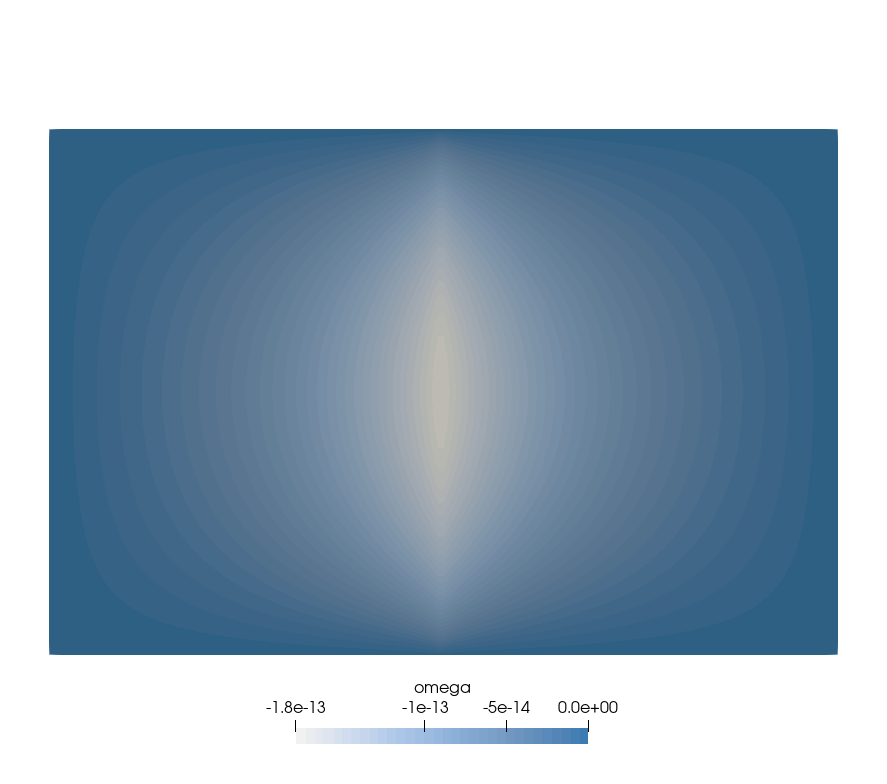
\includegraphics[width=8cm]{python_codes/fieldstone_153/results/exp2/omega}
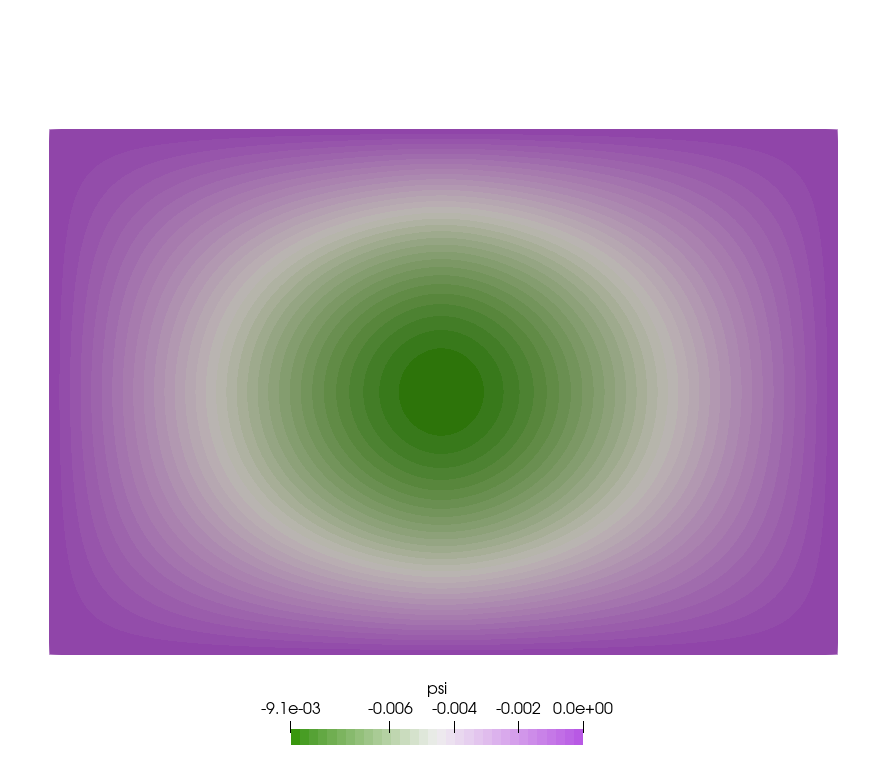
\includegraphics[width=8cm]{python_codes/fieldstone_153/results/exp2/psi}\\
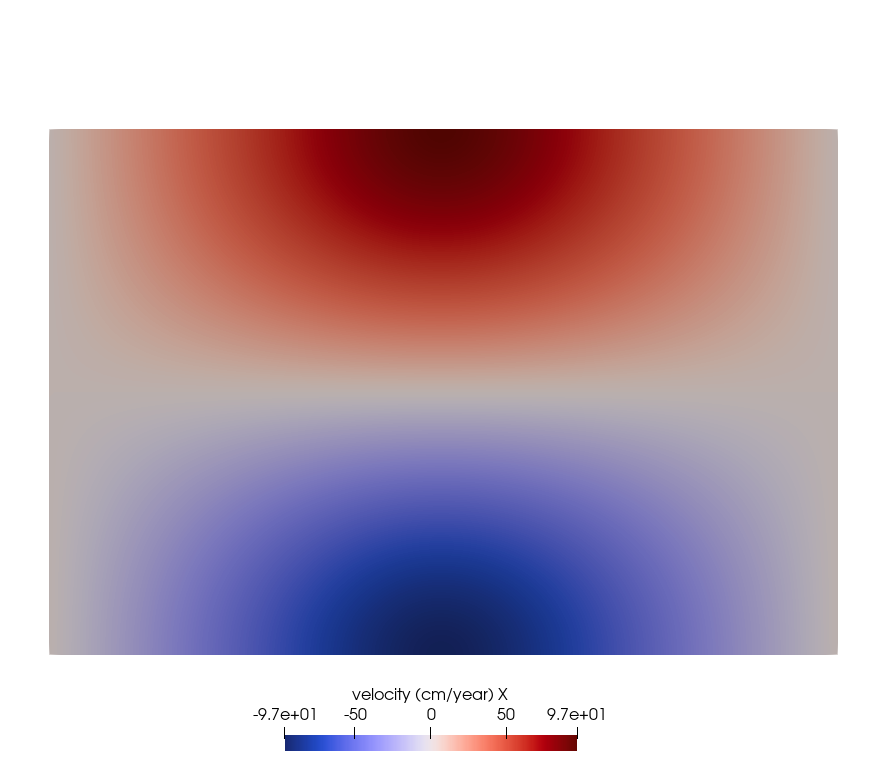
\includegraphics[width=8cm]{python_codes/fieldstone_153/results/exp2/u}
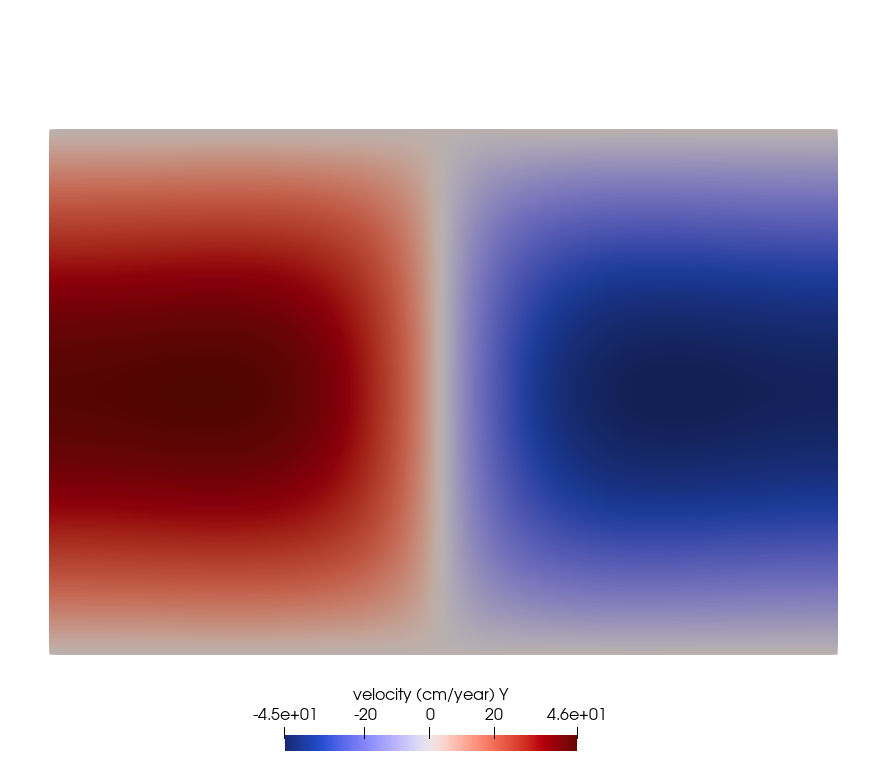
\includegraphics[width=8cm]{python_codes/fieldstone_153/results/exp2/v}\\
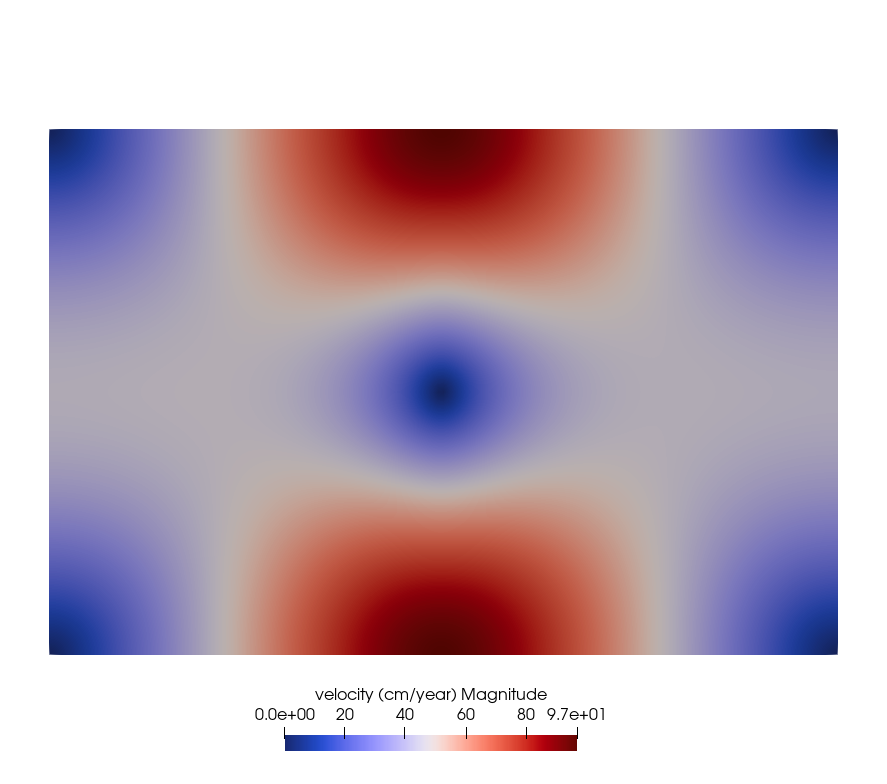
\includegraphics[width=8cm]{python_codes/fieldstone_153/results/exp2/vel}
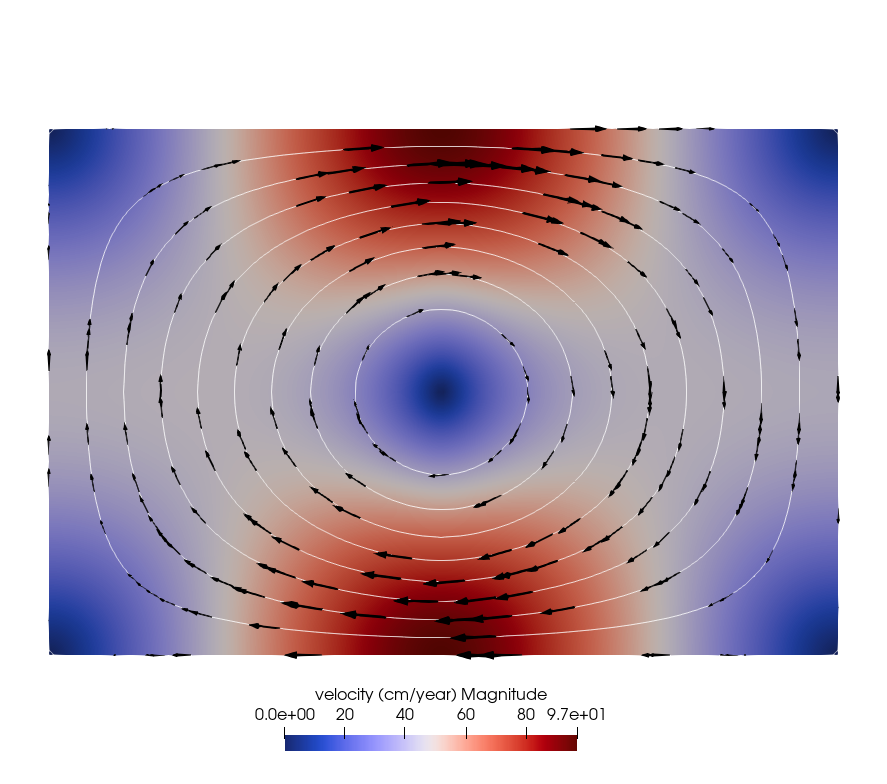
\includegraphics[width=8cm]{python_codes/fieldstone_153/results/exp2/vel2}\\
{\captionfont Top row: $\omega$ and $\Psi$ fields.
Middle row: $u$ and $v$ fields. 
Bottom row: velocity magnitude. Velocity glyphs on $\Psi$ isocontours.}
\end{center}










%%%%%%%%%%%%%%%%%%%%%%%%%%%%%%%%%%%%%%%%%%%%%%%%%%%%%%%%%%%%%%%%%%%%%%%%%%%%%%%%%%%%%%%%%%%%%%%%%%%
\par\noindent\rule{\textwidth}{0.4pt}

\vspace{.5cm}

\begin{center}
\fbox{\begin{minipage}{0.9\textwidth}
{\color{teal}To Do, open questions, future work?}
\begin{itemize}
\item compute pressure via PPE
\end{itemize}
\end{minipage}}
\end{center}



